\subsection{Wellenlängenselektion}

\subsubsection{Selektion über Reflektivität der Spiegel}

\paragraph{Aufbau und Durchführung}
blabla

\paragraph{Auswertung}
blabla

\begin{figure}[H]
\begin{center}
  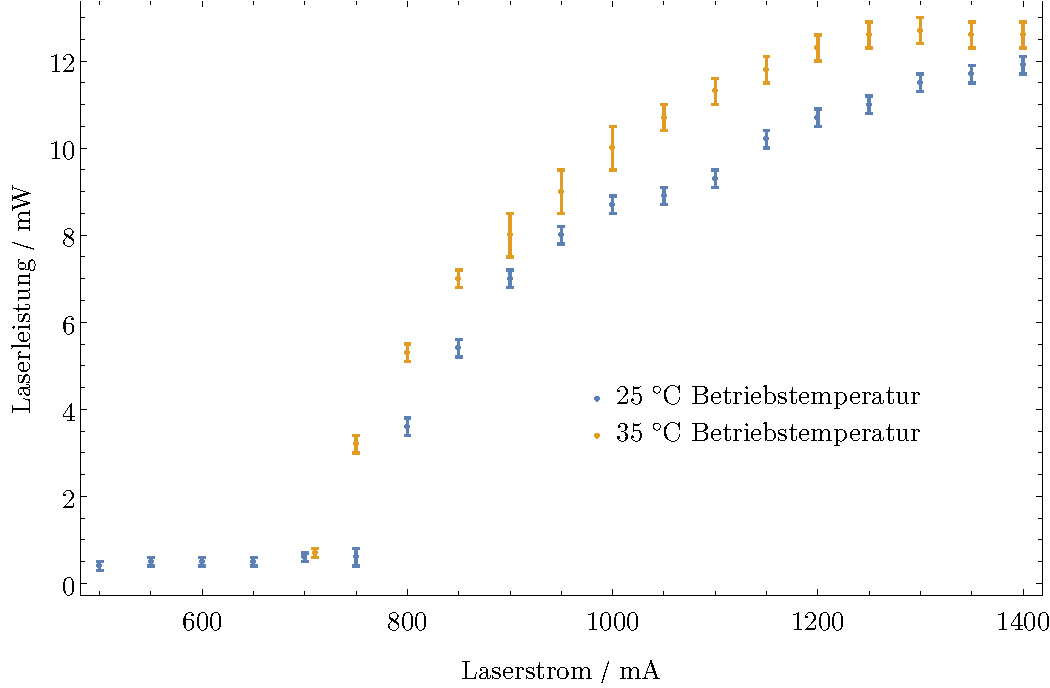
\includegraphics[width=\textwidth]{PI_gruen.pdf}
  \caption{PI-Kennlinie des grünen Lasers bei 25\grad und 35\grad
  Betriebstemperatur.}
  \label{img:PI_gruen}
\end{center}
\end{figure}


\begin{figure}[H]
\begin{center}
  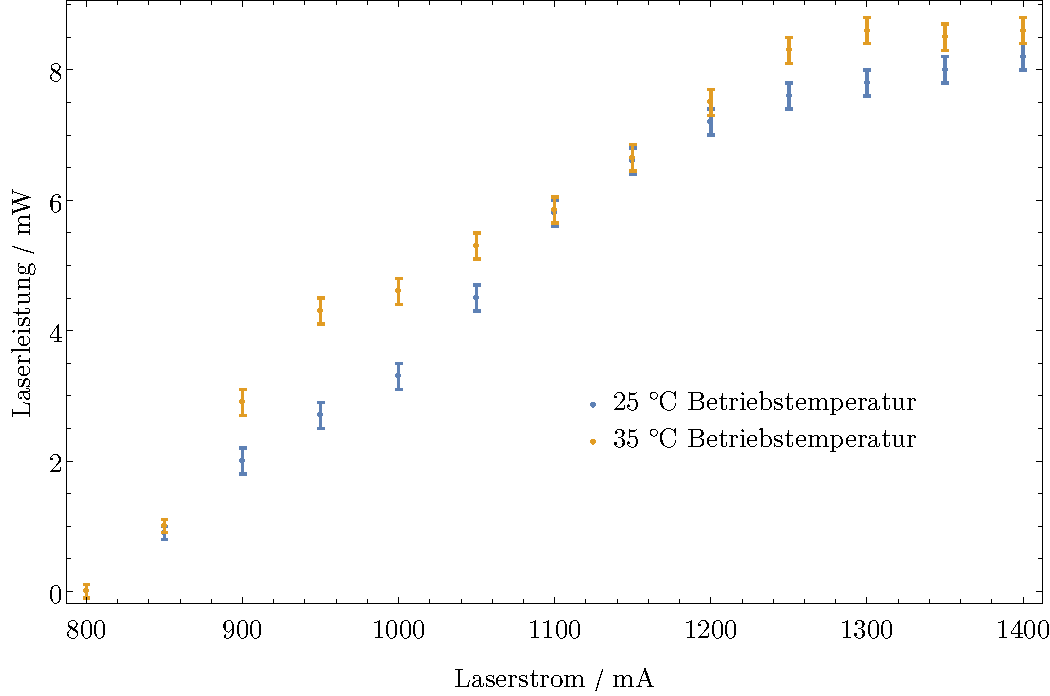
\includegraphics[width=\textwidth]{PI_gelb.pdf}
  \caption{PI-Kennlinie des gelben Lasers bei 25\grad und 35\grad
  Betriebstemperatur.}
  \label{img:PI_gelb}
\end{center}
\end{figure}



\subsubsection{Selektion über doppelbrechenden Kristall}


\paragraph{Aufbau und Durchführung}

\paragraph{Auswertung}

\subsubsection{Selektion mit Littrow-Prisma}


\paragraph{Aufbau und Durchführung}

\paragraph{Auswertung}

